In diesem Kapitel wird eine speziellere Variante der Platzierung von Bildern und Grafiken auf einer Seite gezeigt. Das Einbinden / Anzeigen von einzelnen Bildern ist in den vorhergehenden Kapiteln mehrfach zu sehen.

\vfill

Der \LaTeX-Löwe einmal mit und einmal ohne Rahmen, nebeneinander platziert. 

\begin{figure}[htb]
    \centering
    \begin{minipage}[t]{0.45\linewidth}
        \centering
        
\includegraphics[width=0.9\linewidth]{./Bilder/LaTeX.jpg}
        \caption{\LaTeX-Löwe ohne Rahmen}
    \end{minipage}
    \hfill
    \begin{minipage}[t]{0.45\linewidth}
        \centering
        \fbox{
\includegraphics[width=0.9\linewidth]{./Bilder/LaTeX.jpg}}
        \caption{\LaTeX-Löwe mit Rahmen}
    \end{minipage}
\end{figure}

\vfill

Der \LaTeX-Code für die Platzierung der beiden \LaTeX-Löwen nebeneinander:

\begin{figure}[h!]
    \centering
      \fbox{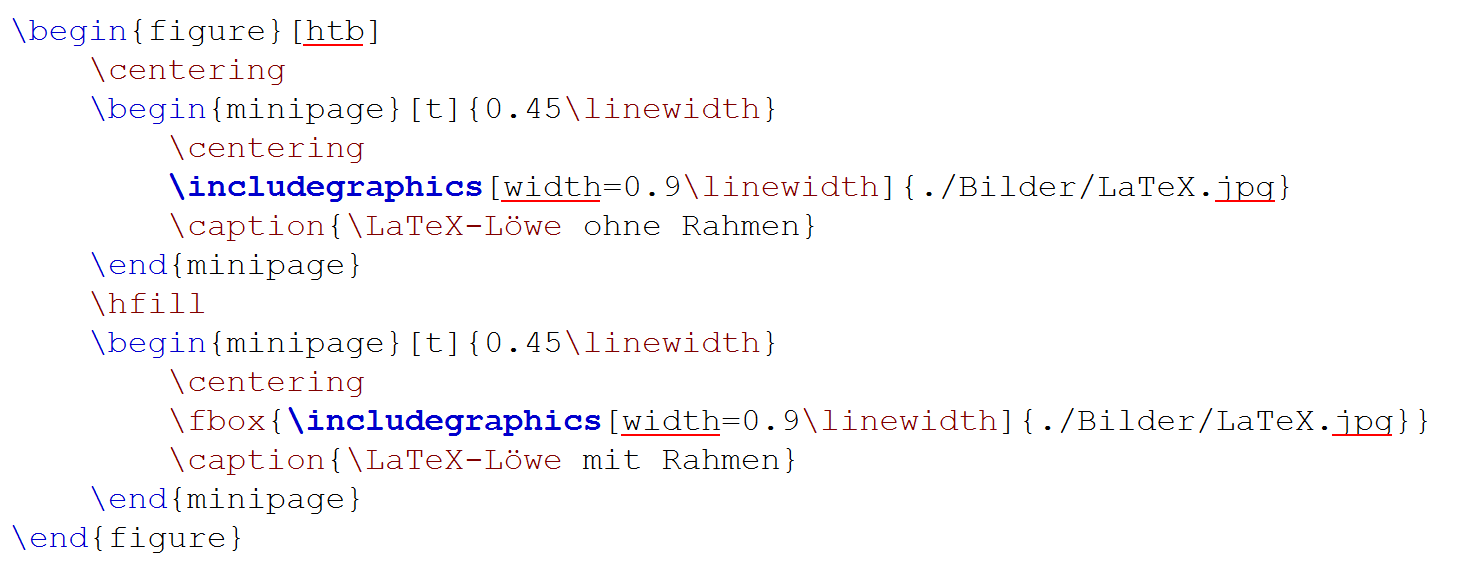
\includegraphics[width=0.9\textwidth]{./Bilder/BilderNebeneinander.png}}  
      \caption{Der \LaTeX-Code zu den beiden \LaTeX-Löwen}
\end{figure}

\vfill

Die vertikale Verteilung über die ganze Seite wird mit \code{\textbackslash{vfill}} erreicht. Der \LaTeX-Code für die Gestaltung der ganzen Seite (inkl. der konkreten Platzierung der \code{\textbackslash{vfill}}) ist in der Tex-Datei zu dieser Seite \code{./Inhalte/Inhalt\_Bilder.tex} zu sehen.

